\documentclass[tikz,border=25pt]{standalone}
\usepackage{amsmath,amssymb}

\begin{document}
	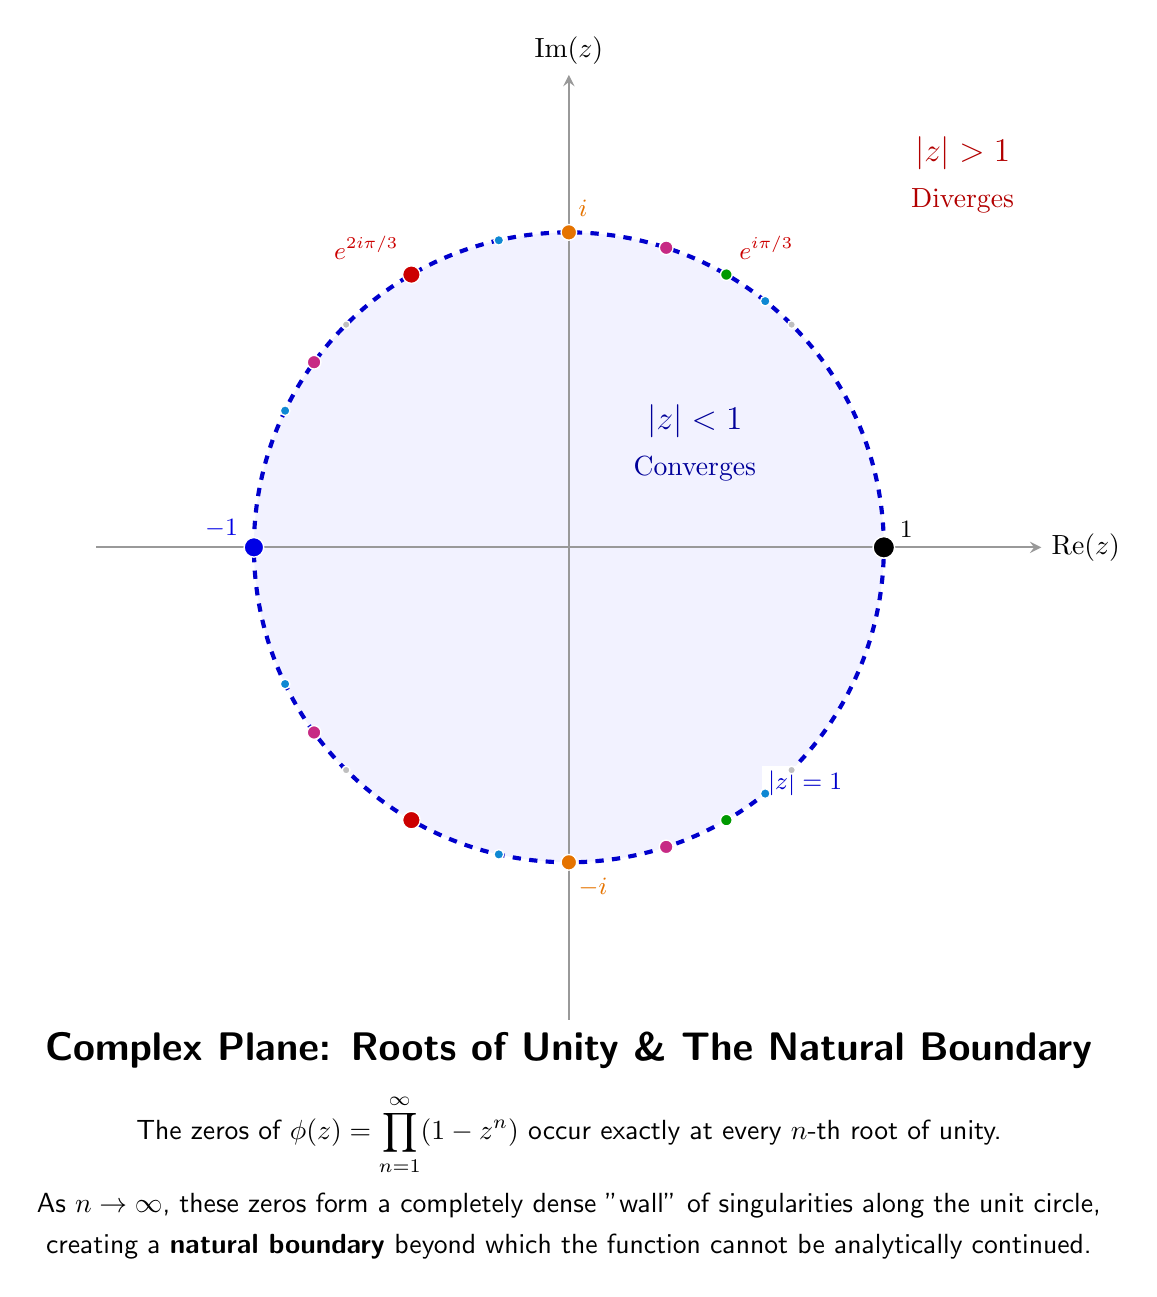
\begin{tikzpicture}[scale=4, font=\sffamily]
		
		% ==========================================
		% AXES & REGIONS
		% ==========================================
		% Draw the shaded region of absolute convergence (|z| < 1)
		\fill[blue!5] (0,0) circle (1);
		
		% Axes
		\draw[thick, ->, >=stealth, gray!80] (-1.5, 0) -- (1.5, 0) node[right, text=black] {$\operatorname{Re}(z)$};
		\draw[thick, ->, >=stealth, gray!80] (0, -1.5) -- (0, 1.5) node[above, text=black] {$\operatorname{Im}(z)$};
		
		% Region labels
		\node[text=blue!60!black, font=\large\bfseries] at (0.4, 0.4) {$|z| < 1$};
		\node[text=blue!60!black, font=\normalsize] at (0.4, 0.25) {Converges};
		\node[text=red!70!black, font=\large\bfseries] at (1.25, 1.25) {$|z| > 1$};
		\node[text=red!70!black, font=\normalsize] at (1.25, 1.1) {Diverges};
		
		% ==========================================
		% THE UNIT CIRCLE (NATURAL BOUNDARY)
		% ==========================================
		\draw[line width=1.5pt, blue!80!black, dashed] (0,0) circle (1);
		\node[fill=white, inner sep=2pt, text=blue!80!black, font=\small\bfseries] at (0.75, -0.75) {$|z| = 1$};
		
		% ==========================================
		% ROOTS OF UNITY (ZEROS OF THE FUNCTION)
		% ==========================================
		% We plot the roots of 1 - z^n = 0 for n = 1 to 8.
		% The loop is reversed so larger dots (smaller n) are drawn last and stay on top.
		
		\colorlet{col8}{gray!50}
		\colorlet{col7}{cyan!70!blue}
		\colorlet{col6}{green!60!black}
		\colorlet{col5}{magenta!80!black}
		\colorlet{col4}{orange!90!black}
		\colorlet{col3}{red!80!black}
		\colorlet{col2}{blue!90!black}
		\colorlet{col1}{black}
		
		\foreach \n in {8, 7, 6, 5, 4, 3, 2, 1} {
			% Calculate dot size: smaller n gets bigger dots
			\pgfmathsetmacro{\dotsize}{3.0 - 0.25*\n}
			
			\foreach \k in {1, ..., \n} {
				\pgfmathsetmacro{\angle}{360 * \k / \n}
				\node[circle, fill=col\n, inner sep=\dotsize pt, draw=white, line width=0.5pt] 
				at (\angle:1) {};
			}
		}
		
		% ==========================================
		% SPECIFIC ROOT ANNOTATIONS
		% ==========================================
		\node[above right, font=\small\bfseries, text=col1] at (0:1.02) {$1$};
		\node[above left, font=\small\bfseries, text=col2] at (180:1.02) {$-1$};
		\node[above right, font=\small\bfseries, text=col4] at (90:1.02) {$i$};
		\node[below right, font=\small\bfseries, text=col4] at (270:1.02) {$-i$};
		\node[above right, font=\small\bfseries, text=col3] at (60:1.02) {$e^{i\pi/3}$};
		\node[above left, font=\small\bfseries, text=col3] at (120:1.02) {$e^{2i\pi/3}$};
		
		% ==========================================
		% TITLE & EXPLANATION
		% ==========================================
		\node[align=center] at (0, -1.9) {
			{\Large \textbf{Complex Plane: Roots of Unity \& The Natural Boundary}} \\[3mm]
			{\normalsize The zeros of $\displaystyle \phi(z) = \prod_{n=1}^\infty (1-z^n)$ occur exactly at every $n$-th root of unity.} \\[2mm]
			{\normalsize As $n \to \infty$, these zeros form a completely dense "wall" of singularities along the unit circle,} \\[1mm]
			{\normalsize creating a \textbf{natural boundary} beyond which the function cannot be analytically continued.}
		};
		
	\end{tikzpicture}
\end{document}